%==============================================================================
% tento soubor pouzijte jako zaklad
% this file should be used as a base for the thesis
% Autoři / Authors: 2008 Michal Bidlo, 2019 Jaroslav Dytrych
% Kontakt pro dotazy a připomínky: sablona@fit.vutbr.cz
% Contact for questions and comments: sablona@fit.vutbr.cz
%==============================================================================
% kodovani: UTF-8 (zmena prikazem iconv, recode nebo cstocs)
% encoding: UTF-8 (you can change it by command iconv, recode or cstocs)
%------------------------------------------------------------------------------
% zpracování / processing: make, make pdf, make clean
%==============================================================================
% Soubory, které je nutné upravit nebo smazat: / Files which have to be edited or deleted:
%   projekt-20-literatura-bibliography.bib - literatura / bibliography
%   projekt-01-kapitoly-chapters.tex - obsah práce / the thesis content
%   projekt-01-kapitoly-chapters-en.tex - obsah práce v angličtině / the thesis content in English
%   projekt-30-prilohy-appendices.tex - přílohy / appendices
%   projekt-30-prilohy-appendices-en.tex - přílohy v angličtině / appendices in English
%==============================================================================
\documentclass[]{fitthesis} % bez zadání - pro začátek práce, aby nebyl problém s překladem
%\documentclass[english]{fitthesis} % without assignment - for the work start to avoid compilation problem
%\documentclass[zadani]{fitthesis} % odevzdani do wisu a/nebo tisk s barevnými odkazy - odkazy jsou barevné
%\documentclass[english,zadani]{fitthesis} % for submission to the IS FIT and/or print with color links - links are color
%\documentclass[zadani,print]{fitthesis} % pro černobílý tisk - odkazy jsou černé
%\documentclass[english,zadani,print]{fitthesis} % for the black and white print - links are black
%\documentclass[zadani,cprint]{fitthesis} % pro barevný tisk - odkazy jsou černé, znak VUT barevný
%\documentclass[english,zadani,cprint]{fitthesis} % for the print - links are black, logo is color
% * Je-li práce psaná v anglickém jazyce, je zapotřebí u třídy použít 
%   parametr english následovně:
%   If thesis is written in English, it is necessary to use 
%   parameter english as follows:
%      \documentclass[english]{fitthesis}
% * Je-li práce psaná ve slovenském jazyce, je zapotřebí u třídy použít 
%   parametr slovak následovně:
%   If the work is written in the Slovak language, it is necessary 
%   to use parameter slovak as follows:
%      \documentclass[slovak]{fitthesis}
% * Je-li práce psaná v anglickém jazyce se slovenským abstraktem apod., 
%   je zapotřebí u třídy použít parametry english a enslovak následovně:
%   If the work is written in English with the Slovak abstract, etc., 
%   it is necessary to use parameters english and enslovak as follows:
%      \documentclass[english,enslovak]{fitthesis}

% Základní balíčky jsou dole v souboru šablony fitthesis.cls
% Basic packages are at the bottom of template file fitthesis.cls
% zde můžeme vložit vlastní balíčky / you can place own packages here

% Kompilace po částech (rychlejší, ale v náhledu nemusí být vše aktuální)
% Compilation piecewise (faster, but not all parts in preview will be up-to-date)
% \usepackage{subfiles}

% Nastavení cesty k obrázkům
% Setting of a path to the pictures
%\graphicspath{{obrazky-figures/}{./obrazky-figures/}}
%\graphicspath{{obrazky-figures/}{../obrazky-figures/}}

%---rm---------------
\renewcommand{\rmdefault}{lmr}%zavede Latin Modern Roman jako rm / set Latin Modern Roman as rm
%---sf---------------
\renewcommand{\sfdefault}{qhv}%zavede TeX Gyre Heros jako sf
%---tt------------
\renewcommand{\ttdefault}{lmtt}% zavede Latin Modern tt jako tt

% vypne funkci šablony, která automaticky nahrazuje uvozovky,
% aby nebyly prováděny nevhodné náhrady v popisech API apod.
% disables function of the template which replaces quotation marks
% to avoid unnecessary replacements in the API descriptions etc.
\csdoublequotesoff



\usepackage{url}
\usepackage[english, czech]{babel}
\usepackage{blindtext}
\usepackage{graphicx}




% =======================================================================
% balíček "hyperref" vytváří klikací odkazy v pdf, pokud tedy použijeme pdflatex
% problém je, že balíček hyperref musí být uveden jako poslední, takže nemůže
% být v šabloně
% "hyperref" package create clickable links in pdf if you are using pdflatex.
% Problem is that this package have to be introduced as the last one so it 
% can not be placed in the template file.
\ifWis
\ifx\pdfoutput\undefined % nejedeme pod pdflatexem / we are not using pdflatex
\else
  \usepackage{color}
  \usepackage[unicode,colorlinks,hyperindex,plainpages=false,pdftex]{hyperref}
  \definecolor{hrcolor-ref}{RGB}{223,52,30}
  \definecolor{hrcolor-cite}{HTML}{2F8F00}
  \definecolor{hrcolor-urls}{HTML}{092EAB}
  \hypersetup{
	linkcolor=hrcolor-ref,
	citecolor=hrcolor-cite,
	filecolor=magenta,
	urlcolor=hrcolor-urls
  }
  \def\pdfBorderAttrs{/Border [0 0 0] }  % bez okrajů kolem odkazů / without margins around links
  \pdfcompresslevel=9
\fi
\else % pro tisk budou odkazy, na které se dá klikat, černé / for the print clickable links will be black
\ifx\pdfoutput\undefined % nejedeme pod pdflatexem / we are not using pdflatex
\else
  \usepackage{color}
  \usepackage[unicode,colorlinks,hyperindex,plainpages=false,pdftex,urlcolor=black,linkcolor=black,citecolor=black]{hyperref}
  \definecolor{links}{rgb}{0,0,0}
  \definecolor{anchors}{rgb}{0,0,0}
  \def\AnchorColor{anchors}
  \def\LinkColor{links}
  \def\pdfBorderAttrs{/Border [0 0 0] } % bez okrajů kolem odkazů / without margins around links
  \pdfcompresslevel=9
\fi
\fi
% Řešení problému, kdy klikací odkazy na obrázky vedou za obrázek
% This solves the problems with links which leads after the picture
\usepackage[all]{hypcap}

% Informace o práci/projektu / Information about the thesis
%---------------------------------------------------------------------------
\projectinfo{
  %Prace / Thesis
  project={BP},            %typ práce BP/SP/DP/DR  / thesis type (SP = term project)
  year={2021},             % rok odevzdání / year of submission
  date=\today,             % datum odevzdání / submission date
  %Nazev prace / thesis title
  title.cs={Generování 2D map pro počítačové hry},  % název práce v češtině či slovenštině (dle zadání) / thesis title in czech language (according to assignment)
  title.en={2D map generation for computer games}, % název práce v angličtině / thesis title in english
  %title.length={14.5cm}, % nastavení délky bloku s titulkem pro úpravu zalomení řádku (lze definovat zde nebo níže) / setting the length of a block with a thesis title for adjusting a line break (can be defined here or below)
  %sectitle.length={14.5cm}, % nastavení délky bloku s druhým titulkem pro úpravu zalomení řádku (lze definovat zde nebo níže) / setting the length of a block with a second thesis title for adjusting a line break (can be defined here or below)
  %dectitle.length={14.5cm}, % nastavení délky bloku s titulkem nad prohlášením pro úpravu zalomení řádku (lze definovat zde nebo níže) / setting the length of a block with a thesis title above declaration for adjusting a line break (can be defined here or below)
  %Autor / Author
  author.name={Kryštof},   % jméno autora / author name
  author.surname={Glos},   % příjmení autora / author surname 
  %author.title.p={Bc.}, % titul před jménem (nepovinné) / title before the name (optional)
  %author.title.a={Ph.D.}, % titul za jménem (nepovinné) / title after the name (optional)
  %Ustav / Department
  department={UPGM}, % doplňte příslušnou zkratku dle ústavu na zadání: UPSY/UIFS/UITS/UPGM / fill in appropriate abbreviation of the department according to assignment: UPSY/UIFS/UITS/UPGM
  % Školitel / supervisor
  supervisor.name={Michal},   % jméno školitele / supervisor name 
  supervisor.surname={Matýšek},   % příjmení školitele / supervisor surname
  supervisor.title.p={Ing.},   %titul před jménem (nepovinné) / title before the name (optional)
  supervisor.title.a={},    %titul za jménem (nepovinné) / title after the name (optional)
  % Klíčová slova / keywords
  keywords.cs={Procedurální generování obsahu, 2D mapy, 2D hry, počítačové hry, hry o přežití}, % klíčová slova v českém či slovenském jazyce / keywords in czech or slovak language
  keywords.en={Procedural content generation, 2D maps, 2D games, computer games, survival games}, % klíčová slova v anglickém jazyce / keywords in english
  %keywords.en={Here, individual keywords separated by commas will be written in English.},
  % Abstrakt / Abstract
  abstract.cs={Procedurální generování se v dnešní době používá v mnoha počítačových hrách a to od 2D RPG her, po 3D FPS. Procedurální generování se používá ve více možných směrech, jako například generování mapy světa, generování okolí světa, za účelem lepšího požitku ze hry a jejího opakovaného hraní. Výsledná hra je žánru Colony-sim inspirovaná hrou RimWorld, je založena na světě generovaným pomocí Perlinova šumu a využívající slabou umělou inteligenci. Praktickým výsledkem je 2D top-down hra vytvořená na platformě Unity založená na procedurálním generování obsahu}, % abstrakt v českém či slovenském jazyce / abstract in czech or slovak language
  abstract.en={Procedural generation is used a lot in today's computer games, from 2D RPG games, to 3D FPS. Procedural generation is used in plenty of aspects, for example world map generation, world surrounding generation, for purpose of more fun from the game and it's replayablility. Result game is colony-sim genre inspired by RimWorld, it is based on world generated using Perlin noise and weak artificial intelligence. Practical result is 2D top-down game build on Unity platform, based on procedural generation of content}, % abstrakt v anglickém jazyce / abstract in english
  %abstract.en={An abstract of the work in English will be written in this paragraph.},
  % Prohlášení (u anglicky psané práce anglicky, u slovensky psané práce slovensky) / Declaration (for thesis in english should be in english)
  declaration={Prohlašuji, že jsem tuto bakalářskou práci vypracoval samostatně pod vedením pana X...
Další informace mi poskytli...
Uvedl jsem všechny literární prameny, publikace a další zdroje, ze kterých jsem čerpal.},
  %declaration={I hereby declare that this Bachelor's thesis was prepared as an original work by the author under the supervision of Mr. X
% The supplementary information was provided by Mr. Y
% I have listed all the literary sources, publications and other sources, which were used during the preparation of this thesis.},
  % Poděkování (nepovinné, nejlépe v jazyce práce) / Acknowledgement (optional, ideally in the language of the thesis)
  acknowledgment={V této sekci je možno uvést poděkování vedoucímu práce a těm, kteří poskytli odbornou pomoc
(externí zadavatel, konzultant apod.).},
  %acknowledgment={Here it is possible to express thanks to the supervisor and to the people which provided professional help
%(external submitter, consultant, etc.).},
  % Rozšířený abstrakt (cca 3 normostrany) - lze definovat zde nebo níže / Extended abstract (approximately 3 standard pages) - can be defined here or below
  %extendedabstract={Do tohoto odstavce bude zapsán rozšířený výtah (abstrakt) práce v českém (slovenském) jazyce.},
  %extabstract.odd={true}, % Začít rozšířený abstrakt na liché stránce? / Should extended abstract start on the odd page?
  %faculty={FIT}, % FIT/FEKT/FSI/FA/FCH/FP/FAST/FAVU/USI/DEF
  faculty.cs={Fakulta informačních technologií}, % Fakulta v češtině - pro využití této položky výše zvolte fakultu DEF / Faculty in Czech - for use of this entry select DEF above
  faculty.en={Faculty of Information Technology}, % Fakulta v angličtině - pro využití této položky výše zvolte fakultu DEF / Faculty in English - for use of this entry select DEF above
  department.cs={Ústav matematiky}, % Ústav v češtině - pro využití této položky výše zvolte ústav DEF nebo jej zakomentujte / Department in Czech - for use of this entry select DEF above or comment it out
  department.en={Institute of Mathematics} % Ústav v angličtině - pro využití této položky výše zvolte ústav DEF nebo jej zakomentujte / Department in English - for use of this entry select DEF above or comment it out
}

% Rozšířený abstrakt (cca 3 normostrany) - lze definovat zde nebo výše / Extended abstract (approximately 3 standard pages) - can be defined here or above
%\extendedabstract{Do tohoto odstavce bude zapsán výtah (abstrakt) práce v českém (slovenském) jazyce.}
% Začít rozšířený abstrakt na liché stránce? / Should extended abstract start on the odd page?
%\extabstractodd{true}

% nastavení délky bloku s titulkem pro úpravu zalomení řádku - lze definovat zde nebo výše / setting the length of a block with a thesis title for adjusting a line break - can be defined here or above
%\titlelength{14.5cm}
% nastavení délky bloku s druhým titulkem pro úpravu zalomení řádku - lze definovat zde nebo výše / setting the length of a block with a second thesis title for adjusting a line break - can be defined here or above
%\sectitlelength{14.5cm}
% nastavení délky bloku s titulkem nad prohlášením pro úpravu zalomení řádku - lze definovat zde nebo výše / setting the length of a block with a thesis title above declaration for adjusting a line break - can be defined here or above
%\dectitlelength{14.5cm}

% řeší první/poslední řádek odstavce na předchozí/následující stránce
% solves first/last row of the paragraph on the previous/next page
\clubpenalty=10000
\widowpenalty=10000

% checklist
\newlist{checklist}{itemize}{1}
\setlist[checklist]{label=$\square$}

% Nechcete-li, aby se u oboustranného tisku roztahovaly mezery pro zaplnění stránky, odkomentujte následující řádek / If you do not want enlarged spacing for filling of the pages in case of duplex printing, uncomment the following line
% \raggedbottom

\begin{document}
  % Vysazeni titulnich stran / Typesetting of the title pages
  % ----------------------------------------------
  \maketitle
  % Obsah
  % ----------------------------------------------
  \setlength{\parskip}{0pt}

  {\hypersetup{hidelinks}\tableofcontents}
  
  % Seznam obrazku a tabulek (pokud prace obsahuje velke mnozstvi obrazku, tak se to hodi)
  % List of figures and list of tables (if the thesis contains a lot of pictures, it is good)
  \ifczech
    \renewcommand\listfigurename{Seznam obrázků}
  \fi
  \ifslovak
    \renewcommand\listfigurename{Zoznam obrázkov}
  \fi
  % {\hypersetup{hidelinks}\listoffigures}
  
  \ifczech
    \renewcommand\listtablename{Seznam tabulek}
  \fi
  \ifslovak
    \renewcommand\listtablename{Zoznam tabuliek}
  \fi
  % {\hypersetup{hidelinks}\listoftables}

  \ifODSAZ
    \setlength{\parskip}{0.5\bigskipamount}
  \else
    \setlength{\parskip}{0pt}
  \fi

  % vynechani stranky v oboustrannem rezimu
  % Skip the page in the two-sided mode
  \iftwoside
    \cleardoublepage
  \fi

  % Text prace / Thesis text
  % ----------------------------------------------
  \ifenglish
    \input{projekt-01-kapitoly-chapters-en}
  \else
    % Autor: Kryštof Glos

\chapter*{Úvod}
Procedurálně vytvářený obsah v herním průmyslu je velmi důležitou součástí her už po několik let. Mnoho her postavených na tomto principu, se již prosadilo na trhu a stále více se uplatňuje. Náhodné vytváření obsahu se používá například na tvoření herních map, věcí v místnosti, skládání různých dopředu vytvořených místností tak aby vznikla jedinečná mapa. Takto implementované hry mají výhodu v opakované hratelnosti a nepředvídatelnosti.

Cílem této práce je návrh a vytvoření prototypu 2D hry, v herním enginu Unity, založené na procedurálním generování herního obsahu. Samotný generační algoritmus pracuje s Perlinovým šumem a výškovými mapami, ty slouží k vytvoření elevace různých bodů na mapě.

Inspirací na téma hry je počítačová hra RimWorld, která se řadí do her typu Colony-sim. Jedná se o žánr, ve kterém hráč ovládá skupinu lidí, kolonii, kterou se snaží, pomocí dobrého vedení, dovést k nějakému danému cíli. V navržené hře je úkolem hráče dostat kolonisty do stavu prosperity a mimo stav nouze o potravu a zdroje. Pohyb kolonistů využívá takzvané NavMesh agenty, kteří spolupracují s vytvořenou navigační sítí (NavMesh).

Vytváření mapy je stěžejní částí celé hry, určuje zdroje pro hráče a tudíž částečně i obtížnost celé hry. Ve hře se objevují nepřátelé, kteří mají jednoduchou umělou inteligenci a jsou jednou z překážek, se kterou se hráč musí během hry vypořádávat. Implementace generačních algoritmů, AI nepřátel a dalšího je popsána v kapitole \ref{implementace}.

Hra je implementována v herním enginu Unity, které je v dnešní době, jedním z nejvíce používaných vývojových nástrojů pro vývoj her. Mezi další oblíbená vývojová prostředí se řadí například, GameMaker, Unreal Engine, Godot. O vývoji v jednotlivých enginech pojednává kapitola \ref{engines}.

Po dokončení implementační části bylo zahájeno experimentování s herními systémy a následovné uživatelské testování. Průběh a výsledky této části práce jsou dále popsány v kapitole \ref{experiments}.

\chapter{Vytváření obsahu v herním světě} 
\label{theory}
Ve světě her jsou dvě možnosti jak přistupovat ke tvoření obsahu, jedním z těchto způsobů je tradiční nebo také \hyperref[traditional]{mechanické}, je jednodušší, vzhledem k tomu že není potřeba žádný algoritmus, ale pracnější. Další možností vytváření obsahu je pomocí metod implementující náhodné nebo také \hyperref[procedural]{procedurální generování obsahu}. 

Hry které mají pouze dvě dimenze se nazývají 2D (z anglického two dimensions). Je mnoho žánrů 2D her, RPG (role playing game) hry na hrdiny s příběhem, strategií, Co-op (kooperační) které jsou postavené na spolupráci více hráčů, survival (hry o přežití), colony-sim (z anglického colonization simulation) které mají simulovat kolonizaci ovládanou hráčem a tak dále. Tato bakalářská práce se zabývá hrou žánru colony-sim. Je mnoho způsobů jak vyvíjet takovou hru, nejčastěji se používají takzvané \hyperref[engines]{herní enginy}, které takové vyvíjení hry ulehčují a jsou na to stavěné.


\section{Způsoby generování obsahu}
V této části porovnáme mechanické generování obsahu s procedurálním, vysvětlíme co je lepší kdy použít a jaké známe metody pro procedurální generování. Následující tři body popisují faktory, které je třeba zvážit při rozhodování, zda bude využita nějaká procedurální metoda generování, nebo bude lepší použít manuální design úrovní a obsahu:
\begin{description}
	\item[Žánr tvořené hry] Při vývoji například takové hry z prvního pohledu (FPS) hry, u které záleží hlavně na ovládání a souboji hráče proti hráči, není třeba vytvářet mapy a další obsah procedurálně. Většinou stačí vytvořit například pouze jednu úroveň a v takovém případě není třeba používat procedurální generování. Při hrách, které závisí na okolí, surovinách a přežití kde každá okolnost nějak ovlivňuje hráče, už procedurální generování hraje větší roli. Zároveň pro vytváření obsahu jako je text, může být PG velmi obtížnou volbou, neboť v RPG hrách bývá textová část velmi důležitá a generování textu je stále dost obtížné
	\item[Opakovaná hratelnost] Některé hry jsou dělané tak, že čím déle hráč hraje stejnou úroveň (anglicky level), tím více se zlepšuje a je za to například odměňován je právě manuální tvoření úrovní lepší než procedurální. Naopak u jiných her, které mají úrovně procedurálně generované, většinou hráč danou úroveň zvládne, pokračuje na další a nepředpokládá se že se k ní bude ještě vracet.
	\item[Aspekt designu hry] Jestliže hra závisí z velké části na jedné úrovni s jejími mechanikami, vlastnostmi a obsahem, pak je lepší ji vytvářet mechanicky a doladit všechny vlastnosti a interakce s hráčem.
\end{description}


\subsection{Mechanické generování obsahu}
\label{traditional}
Mechanický typ generování je jedním z nejobvyklejších tvoření obsahu ve hrách. Používá se převážně v žánrech, jako je RPG (Role Play Game), RTS (Real Time Strategy) a další, ve kterých pozice objektů a struktura mapy hraje velkou roli a bez lidské tvorby by nebylo dosaženo potřebných výsledků. Toto tvoření lze interpretovat jako proces u něhož se návrhář za pomoci různých nástrojů, které postupně aplikuje, snaží dosáhnout požadovaného výsledku. Jde tedy o metodu ručního vytváření obsahu kde designér, nebo grafik navrhuje a postupně vytváří úroveň, či jinou část hry tak, aby vyhovovala potřebám, ať už se jedná o pozici stromu, nebo o to co hráči sděluji NPC.

Díky tomuto přístupu nehrozí nesrovnalosti ve výsledku, například se nemůže stát že určitá část mapy bude nedostupná, nebo úplně nesmyslná. Další výhodou je, že výsledek bude přesně takový jak byl naplánovaný, avšak takovéto tvoření je u větších her, kde je nutná opětovná hratelnost, velmi časově náročné.

\subsection{Procedurální generování obsahu}
Tento typ vytváření obsahu se používá ve více žánrech, ale asi nejznámější z hlediska generování map je Roguelike, kde každá nová hra má unikátní náhodnou mapu. Procedurální generování se ovšem nepoužívá pouze na generování map, ale také na vytváření objektů, jako jsou stromy, textury, animace, text a další. Procedurální generování obsahu není úplně to stejné, jako náhodné generování obsahu. Více do hloubky je tento typ modelování krajiny a textur rozebrán v kapitole \hyperref[procedural]{Procedurální generování}.

V zásadě je to proces obrácený jak u mechanického generování obsahu. Uživatel sice stále definuje různé nástroje, které jsou použity pro vytváření obsahu, ale nikoli pro své vlastní použití, ale naopak je vytváří pro algoritmus. Uživatel dále určuje pravidla podle kterých se generátor musí řídit tak, aby se dobral kýženého výsledku.

\subsubsection{Příklad procedurálního generování lesů}
\label{proceduralExample}
\todo{informace o tom kde konkrétně se používá + obrázky}
Pro lepší představu uvedu příklad. Program má funkci procedurálního generátoru lesů na mapě, cílem tohoto programu je náhodně naskládat stromy s rozumnými rozestupy od sebe. Pomocí mechanického generování obsahu by designér jednoduše přidával modely stromů do té doby, dokud by mapa neodpovídala představám návrháře a nesplňovala by potřeby herního designu. V případě procedurálního generování, je nutné definovat nástroje, což je v tomto příkladě schopnost přidávat stromy na mapu a pravidla, jako například kolik stromů je potřeba aby algoritmus vysázel, kam program může jednotlivé stromy pokládat a jaké jsou minimální rozestupy mezi nimi. Pravidla a nástroje nám tím pádem jednoznačně definují množinu potenciálních výsledku.

\begin{figure}[h]
	\centering
	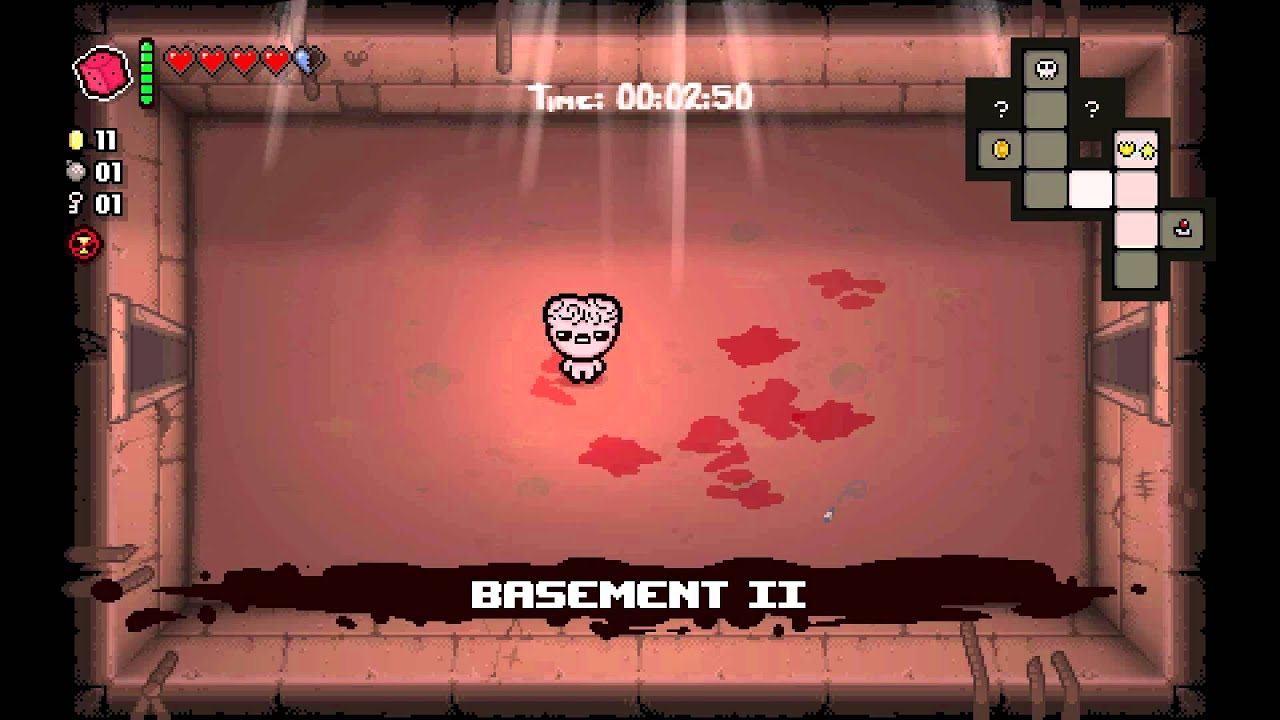
\includegraphics[scale=0.33]{obrazky-figures/BindingOfIsaac.jpg}
	\caption{Příklad hry Roguelike žánru jménem Binding of Isaac, vpravo nahoře je vidět mapa dungeonu, která je procedurálně vygenerovaná.}
\end{figure}


\includegraphics[scale=0.3]{obrazky-figures/keep-calm.png}

\includegraphics[scale=0.3]{obrazky-figures/keep-calm.png}

\todo{dva obrázky, jeden se stromy moc u sebe a druhý lepší při použití více pravidel}

\section{Procedurální generování v herním průmyslu}
\label{proceduralInGames}
Algoritmů na generování obsahu existuje mnoho, každý používá jiné nástroje, ale všechny se musí podrobovat pravidlům která stanovuje programátor a podle kterých se řídí. Je více způsobů a míst kde se dá procedurální generování uplatnit, různé způsoby a důvody jsou popsány v této kapitole.

\subsection{Text}
Skoro všechny hry používají text. Z důvodu že každá informace v textu musí odpovídat realitě, je nutno velké množství omezení pro generování. Například když je v textu informace že král je mrtvý \cite{liuDeep}, musí být toto tvrzení pravdivé.

Velkým plusem procedurálního generování textu je vyprávění \cite{madoc59000}, takto vytvořené příběhy jsou často kreativnější a zajímavější, než ty co by vytvořil člověk, neboť lidé mají sklony psát příběhy které již slyšeli, nebo ze svých zkušeností, což dost omezuje nápady.

\subsection{Krajina a úrovně}
Nejvíce obvyklý obsah který se ve hrách generuje, a který je zároveň hlavním zaměřením této práce, jsou krajiny a úrovně. Generování lokací, úrovní, nebo obsahu mapy lze jak u 2D her, tak u 3D her. Za úroveň nebo oblast lze označovat otevřené, třeba krajina s lesy, i uzavřené prostranství, vnitřek budovy, nebo jeskyně. Tato část PG je rozvedená a podrobněji popsaná v následující kapitole \ref{Krajina}.

\subsection{Textury}
Zároveň se jedná o obsah který má nejméně omezení pro generování. Jednou z nejčastějších metod, která se používá na tvoření textur, je \todo{odkaz na perlinův šum} Perlinův šum, který je detailněji popsán v kapitole \todo{tady a tady}.

\subsection{Zvuky a hudba}
Většina her má soundtrack a zvukové efekty. Soundtrack obvykle nemá nijak zvlášť přísná pravidla, ale zvukové efekty musejí být výstižné a odpovídající akci v daný moment. 

Jukebox \cite{Dhariwal2020JukeboxAG} je model který dokáže generovat hudbu se zpěvem v originální nezpracované formě zvukových dat, s délkou v řádu minut, i s určením žánru a vokálního stylu. Modelů jako je tento již existuje více, avšak zatím to nejsou plně hodnotné soundtracky pro hry a ještě chvíli potrvá, než bude možné jednoduše vygenerovat hudbu a efekty pro hru pomocí pouhého nástroje.

\pagebreak

\chapter{Enginy na vývoj her}
\label{engines}
Herní engine představuje platformu složenou z interagujícího softwaru, který dohromady vytváří integrovaný celek a umožňuje spouštění samotných her. Herní engine se skládá z několika částí s přesně specifikovanou funkcionalitou: rendering, fyzika, síťování, zvuk atd. \cite{nilson2007game} 

Platforem na vývoj her existuje mnoho, některými z nich jsou například Unity, Construct 2, MonoGame, Unreal Engine, nebo GameMaker Studio 2. Každý herní engine je v něčem jiný a tudíž se hodí na jiné žánry, nebo styly her. Při rozhodování, který engine použít, se z hlediska vývojáře musí zohlednit vícero faktorů, například podporovaný programovací jazyk, nebo platformu na kterou je hra vyvíjena. \cite{vohera2021game}
\section{Unity}
\label{unity}

\includegraphics[scale=0.3]{obrazky-figures/keep-calm.png}

\textcolor{gray}{\blindtext[10]}

\chapter{Procedurální generování}
\label{procedural}
Tato kapitola popisuje \todo{konkrétní metody které popisuje} a použití procedurálního generování v herním průmyslu, do detailu popisuje PG krajiny, generování fraktálů.

Procedurální modelování je téma které se aktivně zkoumá už přes čtyřicet let. Myšlenka je, jak již bylo zmíněno, aby obsah který se vytvářel ručně, dal modelovat pomocí navržené procedury automaticky. Takovýto přístup se již uplatnil na generování například textur, geometrických modelů, zvukových nahrávek, nebo animací. V roce 1980 se začalo pracovat s různými metodami na vytváření terénu, jako hory, pláně a jezera. Začal se také řešit růst rostlin a obecně práce s přírodou. \cite{inproceedings}

Roden and Parberry \cite{FromArtistry} pojmenovávají tento druh algoritmů \textit{amplifikační algoritmy (amplification algorithms)}, přijímají menší množství vstupních informací, které zpracují a vracejí větší objem dat na výstupu. Hendrikx et al. \cite{Hendrikx} pojímají procedurální generování jako alternativu k mechanickému navrhování obsahu, ale kladou důraz na zdokonalování a přidávání parametrů umožňujících zásah návrháře do takto vygenerovaných objektů.

\section{Celulární automaty pro PG}
\label{celular}
Celulární automaty se ve hrách používají intenzivně zejména pro modelování týkajícího se systémů v prostředí, jako jsou teplo, oheň, déšť, tlak a exploze. Zatím podle průzkumu nejsou známé žádné hry, které by postavili generování celého 2D herního světa, pouze pomocí celulárních automatů. Momentálně existují webové stránky, které možnost generování malých map pomocí mřížek navrhují, ale není jich mnoho a neexistuje žádné spolehlivé ohodnocení těchto algoritmů. \cite{articleCellular}

Původně byly CA vymyšleny Johnem Von Neumannem jako formální model sebereprodukujících se organismů. Šlo o dvou-dimenzionální celulární automat, kde každá buňka, tzv. cell, je malý čtverec na velkém čtverečkovaném papíru. Každá buňka má dva možné stavy, černý a červený, které jsou určeny jejich sousedstvím. V John Von Neumannově teorii, je sousedství tvořené čtyřmi přilehlými čtverci a na obrázku \ref{vonNeumann} jsou vyznačeny červenou barvou. \cite{Gong2017}

Nejznámější celulární automat byl vytvořen v roce 1970 britským matematikem Johnem Hortonem Conwayem, který se jmenoval Game Of Life. Stejně jako Von Neumannův byl i tento automat dvou-dimenzionální a mohli nabývat pouze hodnot živá, nebo mrtvá. Využívá Moorovo sousedství, které oproti Von Neumannově považuje za sousední buňky všech osm přilehlých, vyobrazené na obrázku \ref{moore}. Fungování automatu je následovné, buňka zůstává naživu, pokud má dvě, nebo tři sousedící buňky živé. Což simuluje, že buňka nepřežije pokud je osamělá, ale zároveň pokud je okolí přeplněné organismy, tak je utlačována. Další pravidlo je, že pokud je libovolná buňka mrtvá, může se "narodit", pokud jsou v sousedství alespoň tři živé buňky. Toto pravidlo má simulovat rození, kde každá buňka musí mít tři rodiče. Automat díky těmto jednoduchým pravidlům dokáže vytvářet simulace které působily jako živý organismus. \cite{Gong2017}

\begin{figure}[h]
	\centering
	\begin{subfigure}{0.475\textwidth}
		\label{vonNeumann}
		\centering
		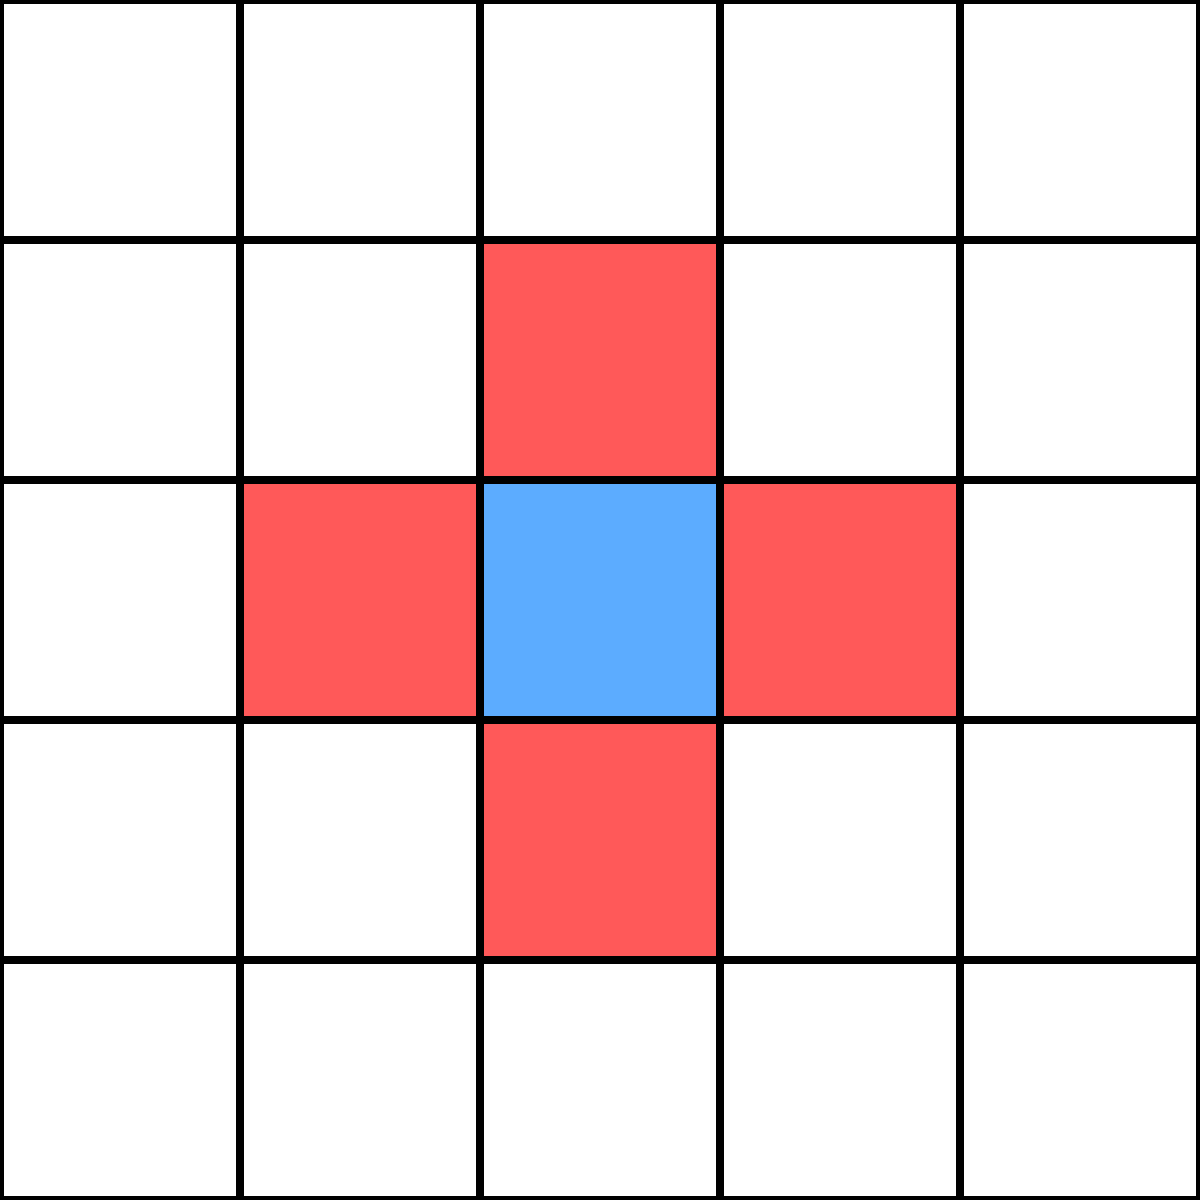
\includegraphics[scale=0.1]{obrazky-figures/Von_neumann_neighborhood.svg}
		\caption{Von Neumannovo sousedství}
	\end{subfigure}
	\begin{subfigure}{0.475\textwidth}
		\label{moore}
		\centering
		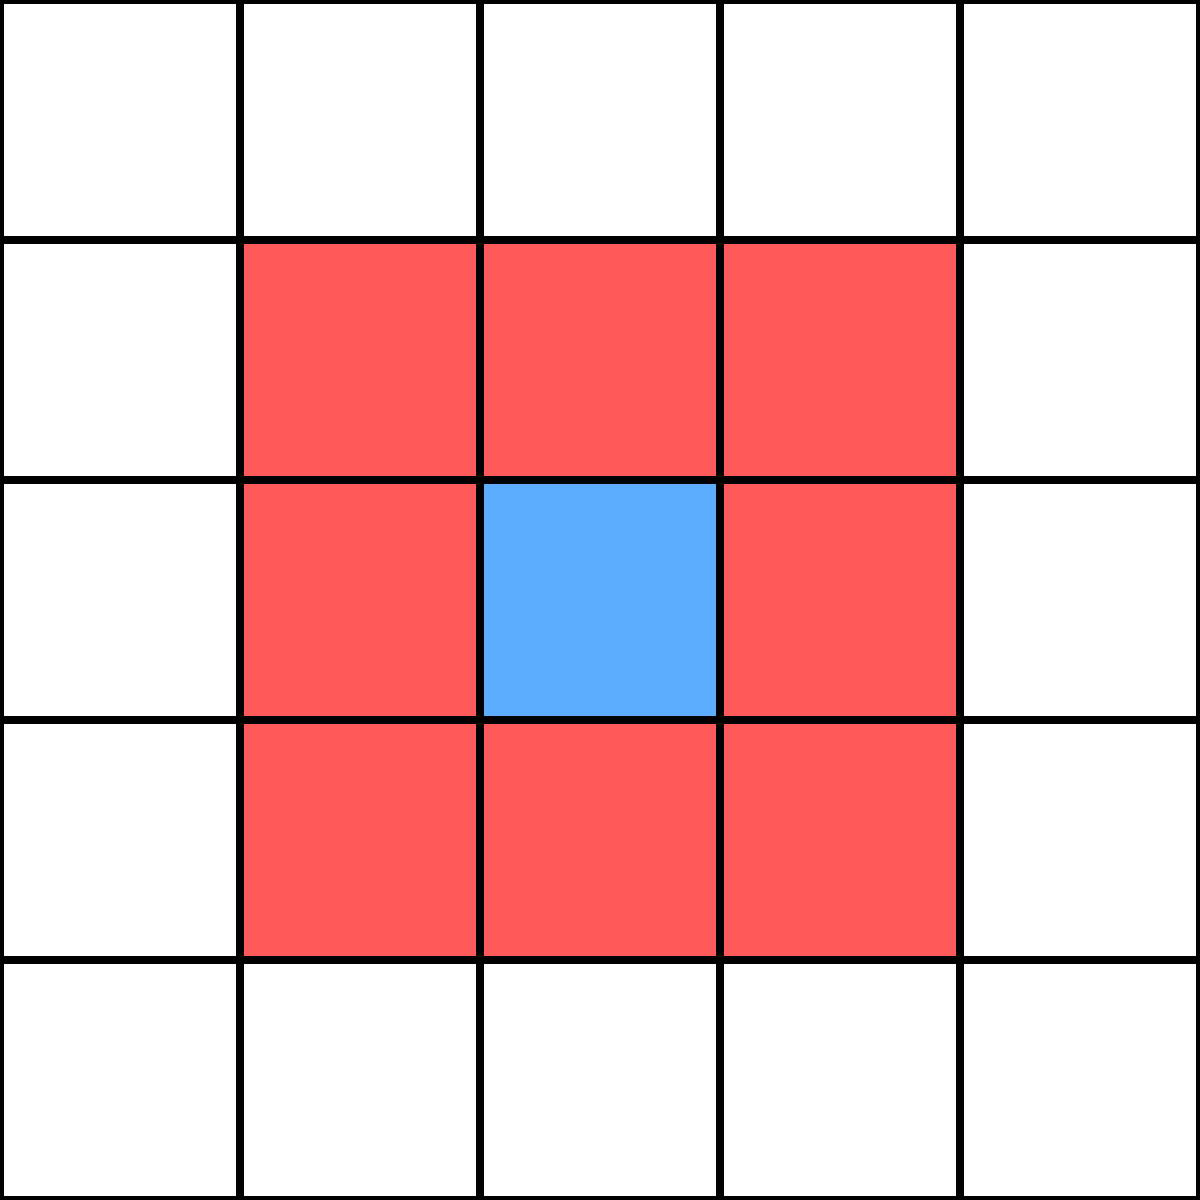
\includegraphics[scale=0.1]{obrazky-figures/Moore_neighborhood.svg}
		\caption{Moorovo sousedství}
	\end{subfigure}
	\caption{Sousedství z pohledu Von Neumanna a Moora}
\end{figure}

\section{Výškové mapy}
\label{heightMaps}
Výškové mapy představují dvoudimenzionální mřížky obsahující výškové hodnoty, jež jsou častým prvkem v modelování terénu. Tyto mapy se běžně využívají jako klíčový prvek pro reprezentaci základu terénu v herním průmyslu. Pro tvorbu výškových map existuje mnoho algoritmů.

Jedny z nejstarších algoritmů jsou metody založené na pododdělení. Segmenty v rámci vygenerované hrubé výškové mapy jsou iterativně rozdělovány, kde každá iterace navíc používá kontrolovanou náhodnost k přidávání detailů. Miller \cite{MillerRendering} popisuje některé varianty všeobecně známé metody středového posunu\todo{napsat něco o této metodě?}, ve které se výška nového bodu nastavuje na průměr hodnot jeho rohů v trojúhelníkovém nebo diamantovém tvaru, k němuž je přidán náhodný offset. Každou iterací se rozsah náhodných hodnot offsetu snižuje, podle parametru, který kontroluje hrubost výsledné výškové mapy. 

Generování výškových map se v dnešní době provádí převážně pomocí fraktálních generátorů šumu, jako je \todo{odkaz na sum}Perlinův šum, který provádí generování šumu vzorkováním a interpolací bodů na mřížce náhodných vektorů.

Výškové mapy se mohou dále transformovat na základě běžných filtrací obrazu, například vyhlazování(smoothing), nebo simulací fyzikálních jevů, např. eroze. \cite{inproceedings}

\section{Procedurální generování krajiny}
\label{terrain}
Procedurální generování krajiny se řadí ke složitějším tématům PG. Je tomu tak hlavně kvůli tomu, že se k tomuto typu generování většinou používají \hyperref[heightMaps]{výškové mapy} (height maps), které se skládají z bitových map odstínů šedé, ve kterých se výška udává pomocí právě odstínu šedé barvy daného pixelu. Většinou se používá postup, při kterém platí, že čím světlejší je pixel, tím větší je výška. Jakmile jsou pixely ohodnoceny, jsou tři různé způsoby jak postupovat:
\begin{itemize}
	\item ruční vykreslování textur,
	\item aplikování textur na ručně vytvořené regiony podle výšky,
	\item vygenerování textur po analyzování výšek na vygenerované výškové mapě.
\end{itemize}
První metoda je výhodná v tom, že textury ručně vykreslené lze udělat na míru a žádný algoritmus je nemůže replikovat. Bohužel jsou časově náročné a jejich kvalita přímo závisí na schopnostech výtvarníka.

Druhá metoda je podobná, nakreslí se barvy na určitá místa, kam si designer myslí že by se mohly hodit hory, řeky, nebo země. Jedná se o docela obvyklou metodu, která přináší velice kvalitní výsledky, ale stále se jedná o manuální techniku.

Třetí metoda používá data height mapy a vypočítává jakou texturu použít na které místo. Nízké hodnoty (tmavší místa) se používají jako oceány, střední hodnoty se vyhodnocují jako země/tráva a na vysoké hodnoty (světlá místa) se nanášejí textury hor nebo kamení. Při generování ve 3D hrách lze ještě započítávat takzvané sklony (slopes), díky kterým je možné oddělovat vyšší plochy od nižších pomocí dalších textur například kamene.

Vzhledem k tomu že první dva postupy vyžadují mechanické vykreslování buď barvy, nebo textur on designéra, nedá se o nich mluvit jako o čistě procedurálních metodách. Naopak postup třetí tomuto popisu zcela odpovídá, neboť kompletně závisí na height mapě a není nutná žádná akce návrháře \cite{madoc59000}.

\pagebreak
\paragraph*{Generování oblastí lze rozdělit následovně:}
\begin{description}
	\item[Vytváření půdorysu] Zahrnuje vytvoření země, moří, řek, hor, atd. Všechny tyto oblasti jsou otevřeného typu. Také můžeme rozumět pod generováním půdorysu i vytváření uzavřeného typu oblastí, například rozložení jednotlivých místností jeskynního komplexu, vytvoření bludiště a jeho cest. 
	
	\item[Přidání vegetace a objektů] Tento bod v podstatě navazuje na předchozí, je potřeba abychom měli vytvořený půdorys, aby bylo kam přidávat a rozmísťovat další objekty. Jedná se o bod do kterého spadá vegetace, budovy, atd. Programu se zadávají různá omezení na množství vegetace, místa kam který objekt lze přidávat a další omezení.
\end{description} 

\begin{figure}[h]
	\centering
	\begin{subfigure}{0.475\textwidth}
		\centering
		
\includegraphics[scale=0.3]{obrazky-figures/keep-calm.png}
		\caption{Vygenerovaný půdorys oblasti}
	\end{subfigure}
	\begin{subfigure}{0.475\textwidth}
		\centering
		
\includegraphics[scale=0.3]{obrazky-figures/keep-calm.png}
		\caption{Přidané stromy k půdorysu}
	\end{subfigure}
	\caption{Na obrázcích jsou vidět různé postupy generování obsahu, na obrázku a je vygenerovaný půdorys oblasti i s mořem a skálou, na obrázku b se k tomu přidaly stromy}
\end{figure}

\todo{informace o všemožných známých metodách procedurálního generování}


\includegraphics[scale=0.3]{obrazky-figures/keep-calm.png}

\section{Metody pro procedurální generování krajiny}
\subsubsection{Porovnání metod}
\todo{porovnání jednotlivých metod}
\textcolor{gray}{\blindtext[8]}


\includegraphics[scale=0.3]{obrazky-figures/keep-calm.png}

\textcolor{gray}{\blindtext[23]}

\section{2D hry}

\todo{popis hry}
\textcolor{gray}{\blindtext[18]}

\includegraphics[scale=0.3]{obrazky-figures/keep-calm.png}

\chapter{Návrh řešení}
\label{solution}
\textcolor{gray}{\blindtext[2]}
\textcolor{gray}{\blindtext[46]}

\section{Vybraná metoda generování}
\todo{podrobnější popis metody, výhody, nevýhody}
\textcolor{gray}{\blindtext[46]}

\chapter{Implementace}
\label{implementace}
Tato část se věnuje podrobnostem implementace skriptů, jež jsou klíčovými součástmi vytváření finální hry.
\textcolor{gray}{\blindtext[60]}
\chapter{Experimenty a vyhodnocení}
\label{experiments}
\section{testování}
\label{tests}
\textcolor{gray}{\blindtext[30]}

\chapter{Závěr}
\label{end}
\textcolor{gray}{\blindtext[4]}
  \fi
  
  % Kompilace po částech (viz výše, nutno odkomentovat)
  % Compilation piecewise (see above, it is necessary to uncomment it)
  %\subfile{projekt-01-uvod-introduction}
  % ...
  %\subfile{chapters/projekt-05-conclusion}


  % Pouzita literatura / Bibliography
  % ----------------------------------------------
\ifslovak
  \makeatletter
  \def\@openbib@code{\addcontentsline{toc}{chapter}{Literatúra}}
  \makeatother
  \bibliographystyle{bib-styles/Pysny/skplain}
\else
  \ifczech
    \makeatletter
    \def\@openbib@code{\addcontentsline{toc}{chapter}{Literatura}}
    \makeatother
    \bibliographystyle{bib-styles/Pysny/czplain}
  \else 
    \makeatletter
    \def\@openbib@code{\addcontentsline{toc}{chapter}{Bibliography}}
    \makeatother
    \bibliographystyle{bib-styles/Pysny/enplain}
  %  \bibliographystyle{alpha}
  \fi
\fi
  \begin{flushleft}
  \bibliography{projekt-20-literatura-bibliography}
  \end{flushleft}

  % vynechani stranky v oboustrannem rezimu
  % Skip the page in the two-sided mode
  \iftwoside
    \cleardoublepage
  \fi

  % Prilohy / Appendices
  % ---------------------------------------------
  \appendix
\ifczech
  \renewcommand{\appendixpagename}{Přílohy}
  \renewcommand{\appendixtocname}{Přílohy}
  \renewcommand{\appendixname}{Příloha}
\fi
\ifslovak
  \renewcommand{\appendixpagename}{Prílohy}
  \renewcommand{\appendixtocname}{Prílohy}
  \renewcommand{\appendixname}{Príloha}
\fi
%  \appendixpage

% vynechani stranky v oboustrannem rezimu
% Skip the page in the two-sided mode
%\iftwoside
%  \cleardoublepage
%\fi
  
\ifslovak
%  \section*{Zoznam príloh}
%  \addcontentsline{toc}{section}{Zoznam príloh}
\else
  \ifczech
%    \section*{Seznam příloh}
%    \addcontentsline{toc}{section}{Seznam příloh}
  \else
%    \section*{List of Appendices}
%    \addcontentsline{toc}{section}{List of Appendices}
  \fi
\fi
  \startcontents[chapters]
  \setlength{\parskip}{0pt} 
  % seznam příloh / list of appendices
  % \printcontents[chapters]{l}{0}{\setcounter{tocdepth}{2}}
  
  \ifODSAZ
    \setlength{\parskip}{0.5\bigskipamount}
  \else
    \setlength{\parskip}{0pt}
  \fi
  
  % vynechani stranky v oboustrannem rezimu
  \iftwoside
    \cleardoublepage
  \fi
  
  % Přílohy / Appendices
  \ifenglish
    \input{projekt-30-prilohy-appendices-en}
  \else
    % Tento soubor nahraďte vlastním souborem s přílohami (nadpisy níže jsou pouze pro příklad)

% Umístění obsahu paměťového média do příloh je vhodné konzultovat s vedoucím
%\chapter{Obsah přiloženého paměťového média}

%\chapter{Manuál}

%\chapter{Konfigurační soubor}

%\chapter{RelaxNG Schéma konfiguračního souboru}

%\chapter{Plakát}

  \fi
  
  % Kompilace po částech (viz výše, nutno odkomentovat)
  % Compilation piecewise (see above, it is necessary to uncomment it)
  %\subfile{projekt-30-prilohy-appendices}
  
\end{document}
